%%%%%%%%%%%%%%%%%%%%%%%%%%%%%%%%%%%%%%%%%
% NIWeek 2014 Poster by T. Reveyrand
% www.microwave.fr
% http://www.microwave.fr/LaTeX.html
% ---------------------------------------
%
% Original template created by:
% Brian Amberg (baposter@brian-amberg.de)
%
% This template has been downloaded from:
% http://www.LaTeXTemplates.com
%
% License:
% CC BY-NC-SA 3.0 (http://creativecommons.org/licenses/by-nc-sa/3.0/)
%
%%%%%%%%%%%%%%%%%%%%%%%%%%%%%%%%%%%%%%%%%

%----------------------------------------------------------------------------------------
%   PACKAGES AND OTHER DOCUMENT CONFIGURATIONS
%----------------------------------------------------------------------------------------

\documentclass[a0paper,portrait]{baposter}

\usepackage[font=small,labelfont=bf]{caption} % Required for specifying captions to tables and figures
\usepackage{booktabs} % Horizontal rules in tables
\usepackage{relsize} % Used for making text smaller in some places

\usepackage{amsmath,amsfonts,amssymb,amsthm} % Math packages
\usepackage{eqparbox}

\usepackage{textcomp}

\usepackage{caption}
\usepackage{subcaption}
\usepackage{graphicx}
\usepackage{listings}
\usepackage{mathtools}

\usepackage{multirow}
%\usepackage{verbatimbox}
%\usepackage{hyperref}

%\usepackage{pgf}

\usepackage[utf8]{inputenc}
\usetikzlibrary{shapes,arrows}
\usepackage{tikz}
\usetikzlibrary{automata,positioning}

\usepackage{multicol}

\usepackage{hyperref}

\usepackage[font=small,labelfont=bf]{caption}

\usepackage{makecell}
\usepackage{enumitem}

\renewcommand\theadalign{bc}
\renewcommand\theadfont{\bfseries}
\renewcommand\theadgape{\Gape[4pt]}
\renewcommand\cellgape{\Gape[4pt]}


\setlist[itemize]{leftmargin=*}

\graphicspath{{figures/}} % Directory in which figures are stored

 \definecolor{bordercol}{RGB}{40,40,40} % Border color of content boxes
 \definecolor{headercol1}{RGB}{210,235,250} % Background color for the header in the content boxes (left side)
 \definecolor{headercol2}{RGB}{210,235,250} % Background color for the header in the content boxes (right side)
 \definecolor{headerfontcol}{RGB}{0,0,0} % Text color for the header text in the content boxes
 \definecolor{boxcolor}{RGB}{240,255,255} % Background color for the content in the content boxes

\tikzset{
    state/.style={
           ellipse,
           draw=black, thin,
           minimum height=0.5cm,
           minimum width=0.6cm,
           text centered,
           font=\scriptsize
           },
    horiz/.style={
           % font=\tiny,
           inner sep=3pt,
           font=\bf

           } ,
    point/.style={
           circle,
           minimum width = 5pt,
           fill
           }
}

\begin{document}

\setlength{\fboxsep}{0pt}

\background{ % Set the background to an image (background.pdf)
\begin{tikzpicture}[remember picture,overlay]
\draw (current page.north west)+(-2em,2em) node[anchor=north west]
{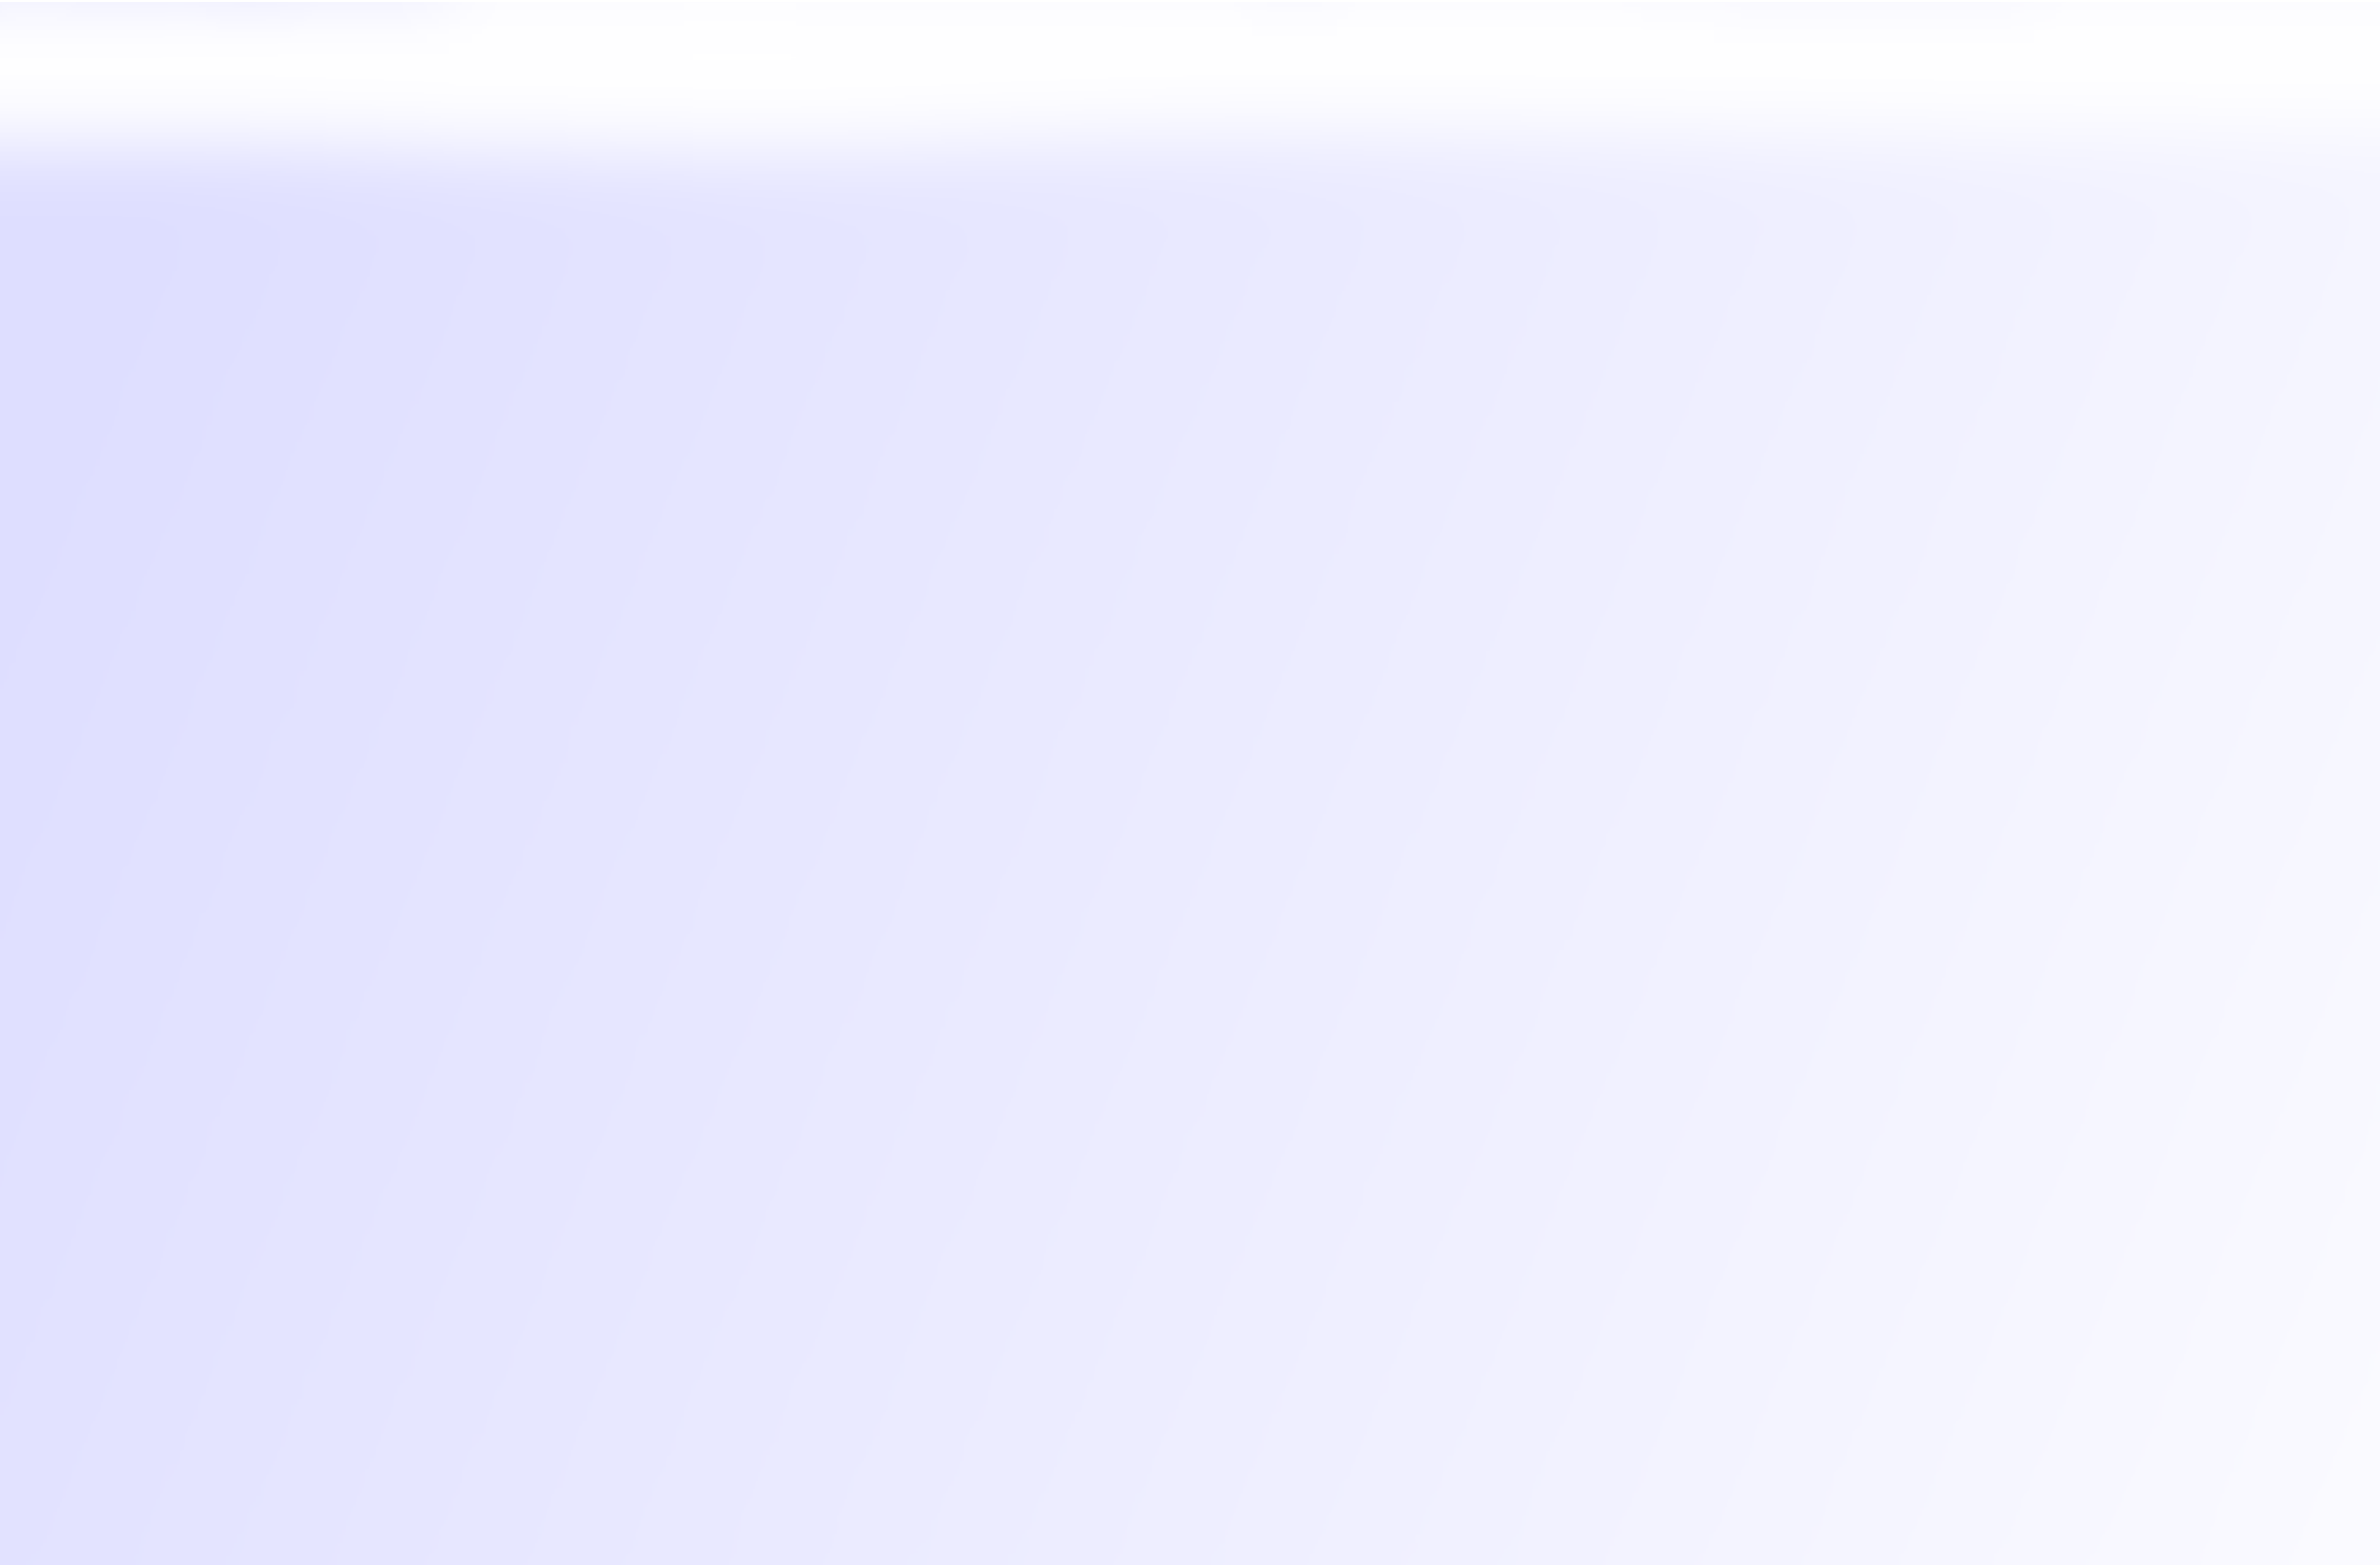
\includegraphics[height=1.1\textheight]{background}};
\end{tikzpicture}
}

\begin{poster}{
grid=false,
columns=12, % because reasons
borderColor=bordercol, % Border color of content boxes
headerColorOne=headercol1, % Background color for the header in the content boxes (left side)
headerColorTwo=headercol2, % Background color for the header in the content boxes (right side)
headerFontColor=headerfontcol, % Text color for the header text in the content boxes
boxColorOne=boxcolor, % Background color for the content in the content boxes
headershape=rectangle, % Specify the rounded corner in the content box headers
headerfont=\Large\sf\bf, % Font modifiers for the text in the content box headers
textborder=none,
background=none,
headerborder=none, % Change to closed for a line under the content box headers
boxshade=plain
}
{
\includegraphics[width=3cm]{sigm0d2.png}}
%
%----------------------------------------------------------------------------------------
%   TITLE AND AUTHOR NAME
%----------------------------------------------------------------------------------------
%
{\bf \huge{Evaluation of \ the Context-Free Path Querying Algorithm Based on Matrix Multiplication} }
%\\  \Large \it Context-free grammars and neural networks for secondary structure} % Poster title
{\vspace{0.6em} \smaller \textbf{Semyon Grigorev} \\  % Author names
\smaller \it {JetBrains Research, Saint Petersburg University, Russia } \\ % Author email addresses
\smaller  {s.v.grigoriev@spbu.ru, Semyon.Grigorev@jetbrains.com}}
{
\includegraphics[width=2.5cm]{SPbGU_Logo.png}} % University/lab logo


%----------------------------------------------------------------------------------------
%   INTRODUCTION
%----------------------------------------------------------------------------------------
\begin{posterbox}[name=CFPQ,column=0,row=0, span=4]{Context-Free Path Querying}

  Find paths which satisfy constraints in form of a formal language $L=\{a^n b^n \mid n > 0\}$
    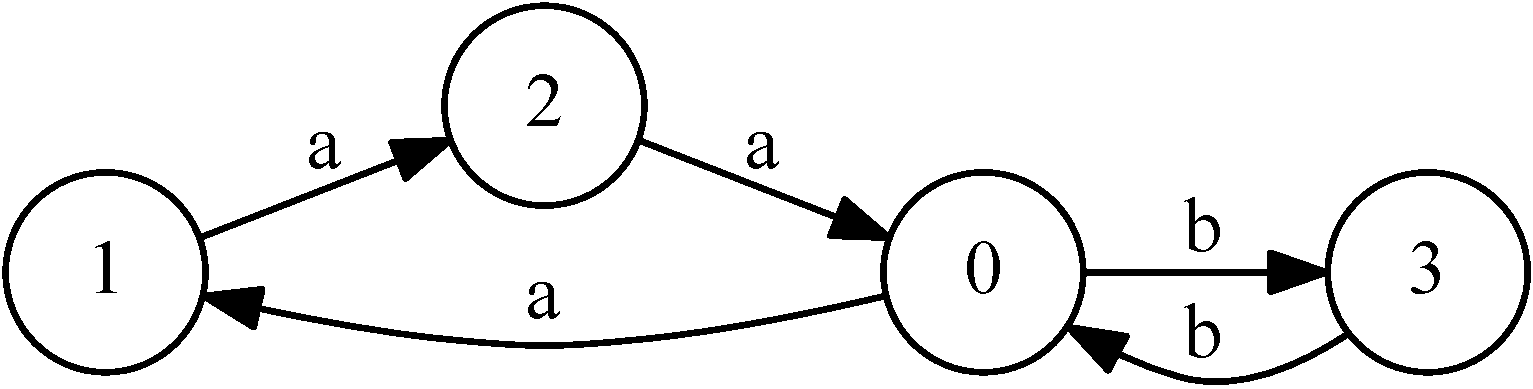
\includegraphics[width=7cm]{example_graph_transparent.png}

    Query = grammar for $L$: $S  \rightarrow a  \ b \ | \ a \ S \ b  \\$

  Result: $ \{(u,v) \mid \exists p \text{ from } u \text{ to } v: \text{word}(p) \in L\} $

\end{posterbox}

\headerbox {Matrix-Based Algorithm~\cite{Azimov:2018:CPQ:3210259.3210264}}
{name=matrices,column=0,span=4, row=2, below=CFPQ}%,bottomaligned=sol2}
{

$T$ is an adjacency matrix of the input graph\\
The grammar is in the normal form
\vspace{-0.5cm}

\begin{align*}
T_{ij} &=\{ N \mid N \xRightarrow[]{*} \omega,  \omega \text{ -- path bw } i \text{ and } j \} \\
T_{ik} \times T_{kj} &= \{ A \mid B \in T_{ik}, C \in T_{kj}, A \rightarrow B C \} \\
T^{(i)} &= T^{(i-1)} \cup (T^{(i-1)} \times T^{(i-1)})
\end{align*}

\begin{itemize}
  \item Can be formulated in terms of boolean \\ matrices multiplication
  \item Easy to run in parallel environments: GPUs, multithreaded CPUs, clusters
%  \item Existing matrix multiplication library can be used
\end{itemize}
\vspace{0.1cm}
}

\headerbox {Results}{name=results,column=4,row=0, span=4, bottomaligned=CFPQ}{
\begin{itemize}
  \item Dataset for CFPQ evaluation is collected and published
  \begin{itemize}
    \item Contains both graphs and queries
    \item Contains both real-world and synthetic graphs
  \end{itemize}
  \item Several CFPQ algorithms implementations are created, evaluated and published
\end{itemize}
}

\headerbox {Future Research}{name=answers,column=8,row=0, span=4, bottomaligned=results}{

\begin{itemize}
  \item Create an open extensible platform for CFPQ \\ algorithms evaluation
  \item Extend dataset with new data
  \item Implement and evaluate distributed \\ matrix-based CFPQ algorithms
  \item Implement and evaluate sparse boolean matrix-based CFPQ algorithms
\end{itemize}

}


\headerbox {Implementations}
{name=impl,column=4,span=8, row=2, below=results,bottomaligned=matrices}
{
\textbf{Our implementations~\cite{Mishin:2019:ECP:3327964.3328503}:}\\
\begin{minipage}[t]{0.6cm}
\hspace{0.6cm}
\end{minipage}
~
\begin{minipage}[t]{0.93\textwidth}
\begin{itemize}
\item[\textbf{[Scipy]}] Matrix-based algorithm which uses sparse matrices from \textbf{Scipy} library (\textbf{Python})
\item[\textbf{[M4RI]}] Matrix-based algorithm which uses dense matrices multiplication from \textbf{m4ri} library (Method of Four Russians, \textbf{C})
\item[\textbf{[GPU]}] Matrix-based algorithm which uses our own implementation of the na\"{\i}ve boolean matrix multiplication in \textbf{CUDA C}
\end{itemize}
\end{minipage}

\vspace{0.5cm}
\textbf{Reference implementations:}\\
\begin{minipage}[t]{1cm}
\hspace{1cm}
\end{minipage}
~
\begin{minipage}[t]{0.91\textwidth}
\begin{itemize}
\item[\textbf{[CuSprs]}] Matrix-based algorithm~\cite{Azimov:2018:CPQ:3210259.3210264} uses NVIDIA cuSPARSE library (\textbf{CUDA C, GPGPU})
\item[\textbf{[CYK]}]  CYK-based algorithm~\cite{10.1007/978-3-319-46523-4_38} implemented in \textbf{Java} (CPU)
  %\item X. Zhang et al, 2016, ``Context-free path queries on RDF graphs''

\end{itemize}

\end{minipage}
}




\headerbox{We Need More Real-World Data}{name=rdfs,span=12,column=0,row=3,below=matrices}{
\vspace{0.05cm}
%\begin{table}[h]
%\rowcolors{1}{}{red}
\begin{minipage}[t]{0.5\textwidth}
Graph: classical ontologies (RDFs)\\
Query: same-generation query over \textbf{\texttt{type}} and \textbf{\texttt{SubClassOf}} relations \\
Grammar: $S \to \textit{scor} \ S \ \textit{sco} \ | \ \textit{tr} \ S \ \textit{t} \ | \ \textit{scor} \ \textit{sco} \ | \ \textit{tr} \ \textit{t}$ \\

\vspace{-0.1cm}

\begin{tabular}{| p{1.5cm} | c | c | c | c | c | c | c |}
    \hline
    \multicolumn{3}{|c|}{RDF}        & \multicolumn{5}{|c|}{Algorithms}  \\
    \hline
    Name                               & \#V & \#E  & Scipy & M4RI & GPU & CuSprs & CYK \\ %~\footnote{Results from X. Zhang et al, 2016, ``Context-Free Path Queries on RDF Graphs''} \\
    \hline
    \hline
    {atm-prim}                    & 291 & 685  & 3 ms     &  2 ms    & 1 ms      & 269 ms  & 8.5 min  \\
    {biomed}                      & 341 & 711  & 3 ms     &  5 ms    & 1 ms      & 283 ms  & 7.1 min  \\
    {pizza}                       & 671 & 2604 & 6 ms     &  8 ms    & 1 ms      & 292 ms  & 54 min \\
    {wine}                        & 733 & 2450 & 7 ms     &  6 ms    & 1 ms      & 294 ms  & 68 min \\
    \hline
  \end{tabular}
%  \captionof{table}{}

\end{minipage}
~
\begin{minipage}[t]{0.48\textwidth}
%\vspace{-1.5cm}
  \begin{itemize}
    \item 2019 (GPU) is $10^6$ times faster than 2016 (CYK) on real-world data
    \begin{itemize}
       \item Reasonable time even for CPU based implementations
    \end{itemize}
    \item We should find bigger RDFs
    \item We should find other real-world cases for CFPQ
    \begin{itemize}
       \item Both graphs and queries
    \end{itemize}

  \end{itemize}
\end{minipage}
}

\setlength{\tabcolsep}{5pt}
\headerbox{We Should Do More Research on the Algorithms Scaling}{name=scaling,span=12,column=0,row=2,below=rdfs}{
\vspace{0.05cm}
\begin{minipage}[t]{0.52\textwidth}

  \begin{tabular}{r | l | c | c | c | c | }
      \cline{2-6}
%      & Graph              & \makecell{Scipy \\ \small sec}  & M4RI      & GPU & CuSprs  \\
      & Graph              & Scipy  & M4RI      & GPU & CuSprs  \\
      \hline
      \hline
      \multirow{4}{3.5cm}{{\small Sparse graphs are generated by GTgraph \\
  Query: $S \to a \ S \ b \ | \ a \ b$}}&
       \small{G10k-0.001} & 37 s  & 2 s    & 0.2 s  & 35 s  \\
      &\small{G10k-0.1}   & 601 s & 1 s    & 0.1 s  & 395 s \\
      &\small{G40k-0.001} & -       & 97 s   & 8.1 s  & -       \\
      &\small{G80k-0.001} & -       & 1142 s & 65 s & -       \\
      \hline
      \hline
      \multirow{3}{3.5cm}{{\small Graph is a cycle \\ Query: $S \to S \ S \ | \ a$}}&
       G25k                & -       & 33 s   & 5 s   & -           \\
      &G50k                & -       & 360 s  & 44 s  & -           \\
      &G80k                & -       & 1292 s & 190 s & -           \\
      \hline
    \end{tabular}
\end{minipage}
~
\begin{minipage}[t]{0.46\textwidth}
\vspace{-2cm}
  \begin{itemize}
    \item We can handle graphs with 80k vertices in a reasonable time by using GPGPU
    \begin{itemize}
     \item Technical bound: GPGPU RAM does not fit bigger graphs
    \end{itemize}
    \item We should evaluate multi-GPU systems
    \item We should evaluate distributed solutions
    \item We should implement a sparse boolean matrices library for GPGPU
   \end{itemize}
\end{minipage}
}



\headerbox {\smaller{Contact Us}}{name=contact,column=0,span=5,below=scaling}{
\scriptsize
\begin{minipage}[t]{0.65\textwidth}
  \vspace{-3cm}
Our team:
\begin{itemize}
  \item Semyon Grigorev: \href{mailto:s.v.grigoriev@spbu.ru}{s.v.grigoriev@spbu.ru}
  \item Nikita Mishin: \href{mailto:mishinnikitam@gmail.com}{mishinnikitam@gmail.com}
  \item Iaroslav Sokolov: \href{mailto:sokolov.yas@gmail.com}{sokolov.yas@gmail.com}
  \item Egor Spirin: \href{mailto:egor@spirin.tech}{egor@spirin.tech}
  \item Egor Nemchinov: \href{mailto:nemchegor@gmail.com}{nemchegor@gmail.com}
\end{itemize}


\end{minipage}
~
\begin{minipage}[t]{3cm}

\includegraphics[width=3cm]{qr-research-jetbra.pdf}
\end{minipage}
\begin{itemize}
  \item Vladimir Kutuev: \href{mailto:vladimir.kutuev@gmail.com}{vladimir.kutuev@gmail.com}
  \item Sergey Gorbatyuk: \href{mailto:sergeygorbatyuk171@gmail.com}{sergeygorbatyuk171@gmail.com}
\end{itemize}
\vspace{1cm}
{\normalsize
Both dataset and implementations are available on GitHub:\\
\url{https://github.com/SokolovYaroslav/CFPQ-on-GPGPU}
}



}

\headerbox{\smaller{References}}{name=references,column=5,span=7,below=scaling}{

    \scriptsize % Reduce the font size in this block
    \renewcommand{\section}[2]{\vskip 0.05em} % Get rid of the default "References" section title
    \nocite{*} % Insert publications even if they are not cited in the poster
    \bibliographystyle{unsrt}
    \bibliographystyle{IEEEtran}
    \bibliography{biblio} % Use biblio.bib as the bibliography file
}

\headerbox {\smaller{Acknowledgments}}{name=ack,column=5,span=7,below=references,bottomaligned=contact}{
\small
The research is supported by the JetBrains Research grant and the~Russian Science Foundation grant 18-11-00100
}


\end{poster}


\end{document}
